
%(BEGIN_QUESTION)
% Copyright 2013, Tony R. Kuphaldt, released under the Creative Commons Attribution License (v 1.0)
% This means you may do almost anything with this work of mine, so long as you give me proper credit

Examine this process trend showing the PV (red), SP (blue), and Output (green) of a loop controller:

$$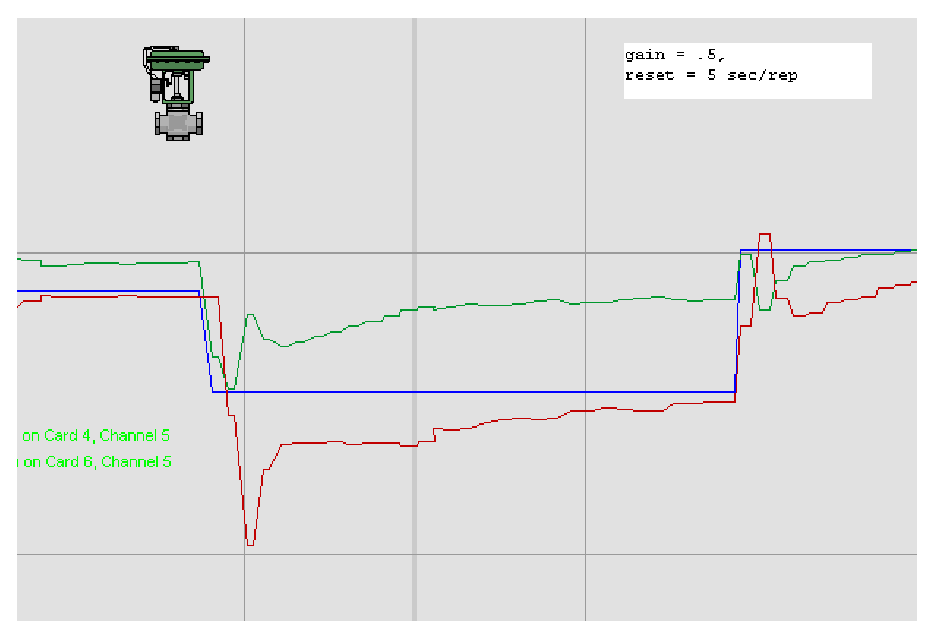
\includegraphics[width=15.5cm]{i02643x01.eps}$$

Based on what you see here, determine the following:

\begin{itemize}
\item{} Whether this is an open-loop or a closed-loop response
\item{} Whether the controller is (or needs to be) {\it direct-acting} or {\it reverse-acting}
\item{} If possible, identify any problems with the field instrumentation
\item{} If possible, identify any problems with the controller PID tuning
\item{} Qualitatively identify the kind of PID tuning we will need for robust control
\end{itemize}

\underbar{file i02643}
%(END_QUESTION)





%(BEGIN_ANSWER)

This is a {\it closed-loop test}, based on the fact the output signal responds dynamically to the changing process variable, as well as to the step-change in setpoint.

\vskip 10pt

This is a {\it reverse-acting} controller: the output steps up when the setpoint steps up (implying the output would step down if the process variable stepped up).

\vskip 10pt

One feature evident in this trend is some final control element hysteresis (e.g. a ``sticky'' control valve).  The evidence of valve stiction is the different process gains ($\Delta \hbox{PV} \over \Delta \hbox{Output}$) when the valve changes direction!  We know this is probably not due to process gain variability because this marked process gain change happens at similar PV values.

\vskip 10pt
  
The controller tuning is clearly too aggressive for this process.  Note the ``porpoising'' action of the PV as it approaches SP following the SP step-change.  Only two types of controller action can cause this to occur: {\it proportional}, or {\it derivative}.  Porpoising is when an oscillation occurs in the PV prior to it crossing setpoint, which explains why integral action cannot ever be to blame for porpoising: the only way a loop oscillation can occur is when the final control element oscillates as well (i.e. changes direction), and since integral action will never change direction until PV crosses SP, oscillations that occur on one side of SP cannot be caused by integral action.  It would appear that the culprit is proportional action (gain), given the 180$^{o}$ phase shift between PV and output following SP step-changes.  It is also clear that more integral action could be used -- it appears as though the person who tuned this was trying to control the process mostly with proportional, even though the tuning parameters (gain = 0.5 and reset = 5 seconds/repeat) actually appears heavily weighted toward reset action.

\vskip 10pt

This is definitely a self-regulating process, as revealed by the fact a new output value is required to achieve a new setpoint value.  This means integral control action will definitely be necessary.  More integral action (reset less than 5 seconds per repeat) and less proportional action (gain lower than 0.5) is what we need here.

%(END_ANSWER)





%(BEGIN_NOTES)


%INDEX% Process troubleshooting: diagnosing problem via trend recording

%(END_NOTES)


